\chapter{Návrh architektury}

Bylo zamýšleno, že klientská aplikace bude komunikovat se serverovou částí, která bude stahovat data z různých datových zdrojů a výsledky posílat zpět klientské aplikaci. Ta v případě potřeby bude stahovat přímo z internetu obrázky, pokud na ně uzly odkazují. Idea rozdělení klienta a serveru byla v tom, že v budoucnu může být na serveru implementováno chachování, aby aplikace byla plynulejší a neprobíhalo zatěžování datových zdrojů.\footnote{Při příliš rychlém stahování z Wikidat lze bohužel snadno dostat IP ban, tedy alespoň pro Wikipedii je cachování nezbytné.}

Server tak slouží na odstínění od link datové vrstvy a v budoucnu pro cachování dat.

Chachování aktuálně implementováno ještě není, server je tedy kompletně bezestavový.

\begin{figure}[h]
    \centering
    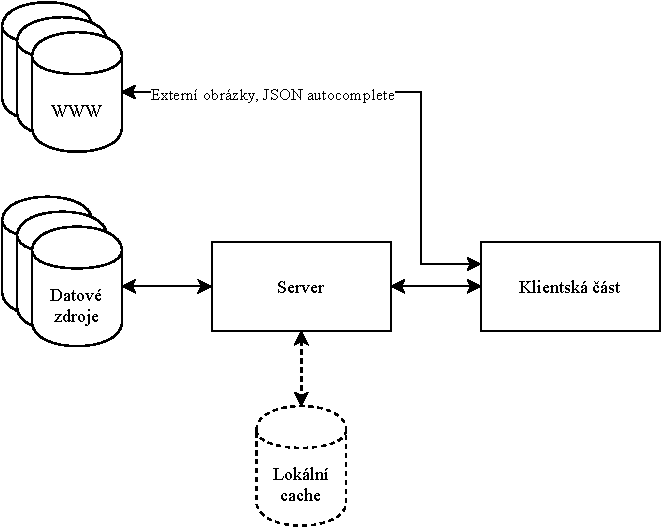
\includegraphics[width=0.75\textwidth]{media/communication.pdf}
    \caption{Komunikace mezi klientem, serverem a datovými zdroji. Cachování na serveru ještě implemontováno není.}
\end{figure}



\section{Server}
Jak již bylo zmíněno dříve, převážná část serveru byla napsána mým vedoucím Martinem Nečaským a sloužila i jako technická specifikace pro klientsou část. Server je napsaný v JavaScriptu a běží v Node.js\footnote{\url{https://nodejs.org/}}. Server je bezestavový a odpovídá na požadavky zmíněné dále.

\subsection{Jazyková podpora}
Server jsem částečně přepsal, aby podporoval dotazování na data z více světových jazyků. Některé požadavky přijímají parametr \texttt{languages} obsahující čárkou (\texttt{,}) oddělené ISO 639-1 jazykové kódy. Server pak vrací objekty jejiž klíčem je jazykový kód a hodnotou daný překlad do jazyka. Pokud překlad neexistuje, hodnotou je \texttt{null}. V případě, že na všechny jazyky bylo vráceno \texttt{null}, server se pokusí přidat další jazyk, který existuje. Který jazyk takto bude vybrán není určeno.

\begin{prikl}
Pro \texttt{languages=cs,en} může server vrátit například
\begin{code}[frame=none]
{
    cs: null,
    en: "Kankakee County"
}
\end{code}
ale pokud nezná překlad ani do češtiny, ani do angličity, může vrátit
\begin{code}[frame=none]
{
    cs: null,
    en: null,
    sk: "Jazero Beňatina"
}
\end{code}
\end{prikl}

\subsection{API}
Server vrací data ve formátu JSON, požadavky jsou posílány metodou GET a parametry jsou kódovány do URL adresy.

\subsubsection{/metaconfiguration}
\textbf{parametry:} \texttt{iri} a \texttt{languages} \\
Vrátí informace o metakonfiguraci zadané podle \texttt{iri}. \\
Vrátí všechna data (viz kapitola \ref{pozadavky-metakonfigurace}) o metakonfiguraci, veškerá data o dceřiných konfiguracích (viz kapitola \ref{pozadavky-konfigurace}) a základní data o dceřiných metakonfiguracích (vše kromě seznamu konfigurací a metakonfigurací).

\begin{code}
interface ResponseMetaConfiguration extends
ResponseMetaConfigurationBase {
    has_meta_configurations: ResponseMetaConfigurationBase[],
    has_configurations: ResponseConfiguration[],
}

interface ResponseMetaConfigurationBase {
    iri: string,
    title: {[language: string]: string},
    description: {[language: string]: string},
    image: string,
}
\end{code}

\subsubsection{/configuration}
\textbf{parametry:} \texttt{iri} a \texttt{languages} \\
Vrátí informace o konfiguraci zadané podle \texttt{iri}. \\
Vrátí stejná data jako \texttt{/metaconfiguration} o svých sceřiných konfiguracích. \\
Toto volání se používá pouze když uživatel ručně zvolí IRI konfigurace, v opačném případě si aplikace vystačí s voláním \texttt{/metaconfiguration}.

\begin{code}
interface ResponseConfiguration {
    iri: string,
    stylesheet: string[],
    title: {[language: string]: string},
    description: {[language: string]: string},
    autocomplete: string[],
    starting_node: string[],
    resource_pattern: string|null,
}
\end{code}

\subsubsection{/stylesheet}
\textbf{parametry:} \texttt{stylesheet} \\
Vrátí kompletní visual style sheet (viz kapitola \ref{pozadavky-visual-style-sheet}) na základě jeho IRI jako parametr \texttt{stylesheet}.

\begin{code}
interface ResponseStylesheet {
    styles: {
        selector: string;
        properties: {
            [property: string]: string;
        }
    }[];
}
\end{code}

\subsubsection{/view-sets}
\textbf{parametry:} \texttt{config} a \texttt{resource} \\
Vrátí seznam možných view setů (viz kapitola \ref{pozadavky-view-sets}) které odpovídají uzlu s IRI \texttt{resource} při dané konfiguraci \texttt{config}.

\begin{code}
interface ResponseViewSets {
    viewSets: {
        iri: string;
        label: string;
        defaultView: string;
        views: string[];
    }[];
    views: {
        iri: string;
        label: string;
    }[];
}
\end{code}

\subsubsection{/preview}
\textbf{parametry:} \texttt{view} a \texttt{resource} \\
Vrátí data z dotazu preview (viz kapitola \ref{pozadavky-preview}) na uzel s IRI \texttt{resource} při daném pohledu \texttt{view}.

\begin{code}
interface ResponsePreview {
    nodes: ResponseElementNode[];
    types: ResponseElementType[];
}
\end{code}

\subsubsection{/detail}
\textbf{parametry:} \texttt{view} a \texttt{resource} \\
Vrátí data z dotazu detail (viz kapitola \ref{pozadavky-detail}) na uzel s IRI \texttt{resource} při daném pohledu \texttt{view}.

\begin{code}
interface ResponseDetail {
    nodes: {
        iri: string;
        data: {
            [IRI: string]: string;
        };
    }[];
    types: ResponseElementType[];
}
\end{code}

\subsubsection{/expand}
\textbf{parametry:} \texttt{view} a \texttt{resource} \\
Vrátí expandované uzly (viz kapitola \ref{pozadavky-expansion}) pro uzel s IRI \texttt{resource} při daném pohledu \texttt{view}. Tyto expandované uzly již obsahují data o detailu a tedy není třeba žádného dalšího volání.

\begin{code}
interface ResponseExpand {
    nodes: ResponseElementNode[];
    edges: ResponseElementEdge[];
    types: ResponseElementType[];
}
\end{code}

\newpage

Mezi pomocná rozhraní pak patří
\begin{code}
interface ResponseElementType {
    iri: string;
    label: string;
    description: string;
}

interface ResponseElementEdge {
    source: string;
    target: string;
    type: string;
    classes: string[];
}

interface ResponseElementNode {
    iri: string;
    type: string;
    label: string;
    classes: string[];
}
\end{code}


\section{Klient}
